\documentclass[a4paper]{article}

\usepackage[natbib=true,style=authoryear-comp,backend=biber,doi=false,url=false,isbn=false]{biblatex}
\bibliography{paper}

\usepackage{todonotes}
\usepackage{a4wide}
\usepackage{amsmath}
\usepackage{amssymb}
\usepackage{syllogism}
\usepackage{subcaption}


\usepackage{xcolor}
\definecolor{Red}{RGB}{178,34,34}
\newcommand{\mf}[1]{\textcolor{Red}{[mf: #1]}}

\begin{document}

\title{Natural sources of vagueness and their implications}
\author{Jos\'e Pedro Correia \and Michael Franke}
\date{}

\maketitle

\begin{abstract}
A vexing puzzle about vagueness, rationality and evolution runs, in crude abbreviation, as follows: vague language use is demonstrably suboptimal if the goal is efficient precise and cooperative information transmission; hence rational deliberation or evolutionary selection should, under this assumed goal, eradicate vagueness from language use.
Since vagueness is persistent in all human languages, something has to give.
In this paper, we investigate a number of reasons why and mechanisms how vagueness may come into the picture in formal models of rational or evolutionary optimal signaling.
We show how uncertainty about not only the linguistic practices of others, but also about the world itself can lead to vagueness, and how, given vagueness, natural linguistic practices are likely to create more reason for vagueness.
We explore the consequences of these reasons and mechanism for a notion of meaning and a notion of language.
\end{abstract}

\tableofcontents

\section{Vagueness}
\label{sec:vagueness}

The classic philosophical problem of vagueness is most starkly embodied by the sorites paradox.
The original formulation is attributed to Eubulides, an ancient Megarian philosopher~\parencite{sorensen_sorites_2009}, and uses the example of a heap of sand: if no removal of one grain of sand can make a heap into a non-heap, we can repeatedly remove all but one grain of sand of something that is clearly a heap and be forced to acknowledge that the remaining single grain of sand is still a heap; otherwise, it seems, we would have to accept that there is a determinate number of grains that forms a heap, and anything under it is not a heap.
Neither choice is, however, intuitively satisfying.
The paradox is interesting because it can be made general and re-applied to many other words besides `heap'.
Predicates for which one can find a suitable instance of the general formulation of the sorites paradox are called \emph{vague}.
Paradigmatic examples besides `heap' include `tall', `red', `bald', `tadpole', and `child'~\parencite{Keefe1997}.
How widespread is the problem?
It is easy to come up with more examples of predicates based on more finely grained properties---as `tall' is intuitively based on height---for which constructing a sorites paradox would be easy.
Mereological nihilists argue that instances of the sorites can be designed for any material object that can be decomposed into small enough parts.
If we subscribe to the scientific picture of matter as composed of molecules and atoms, this applies to tables and chairs, cats and mats, and any other ordinary thing~\parencite{Unger1979}.
Bertrand Russell famously argued~\parencite*{russell_vagueness_1923} that all words, including ``the words of pure logic'', are vague when used by human beings.
The problem thus seems to be a serious one.
But it does not obviously undermine our everyday practices, so the issue must be with the conceptions we have of the mechanisms that underlie them.

Vagueness is typically seen as a challenge to the classical conception of language and meaning.
One problem is that vague predicates seem to lack precise boundaries; if that is the case, how can words like `tall' stand in correspondence to something like a well defined set of tall people?
And if we cannot know exactly whether a certain person is `tall' or not, as with borderline cases, how are we to determine the truth value of sentences that involve statements of tallness regarding these borderline cases?
Supervaluationism, many-valued logics, and degree theories all propose changes to the classical picture in order to accommodate for vague predicates.
They are, however, still strongly committed to retaining as much as possible of it, particularly the core notions of truth and reference.
Mark Sainsbury~\parencite*{sainsbury_concepts_1999} argues that, because of that, they all fail to address an important characteristic of vague predicates: \emph{higher order vagueness}.
All the aforementioned proposals end up being committed to new artificial demarcating boundaries (\emph{e.g.}~true-under-all-precisifications versus neither true nor false versus false-under-all-precisifications, true versus indefinite versus false, true to degree 1 versus true to degree 0 versus the rest).
But a vague predicate not only fails to demarcate between the cases where it clearly applies and the ones where it clearly doesn't, it also fails to establish a boundary between the cases where it clearly applies and the borderline cases, as well as between the borderline cases and the cases where it clearly doesn't apply.
Further introducing borderline borderline cases would lead into an infinite regress.
Because of their attachment to the classical picture, the standard approaches to vagueness fail to see an important lesson, namely that ``we do not know, cannot know, and do not need to know these supposed boundaries to use language correctly''~\parencite*[256]{sainsbury_concepts_1999}.
% \begin{quote}
% But to what in our actual use of language does this division correspond?
% It looks as if, as before, it should correspond to the sentences true beyond the shadow of vagueness, those in some kind of borderline position, and those false beyond the shadow.
% But [\ldots] we do not know, cannot know, and do not need to know these supposed boundaries to use language correctly.
% Hence they cannot be included in a correct description of our language.%
% ~\parencite[256]{sainsbury_concepts_1999}
% \end{quote}
By trying to cling as much as possible to the classical picture of logic and semantics, these standard approaches are ignoring a simple observation: natural language users are sensitive to the sorites paradox, \emph{i.e.}~are able to recognize the logical inconsistency but do not have a good answer to overcome it.
Even more importantly, they apparently do not need to solve the inconsistency in order to continue using natural language productively.
Nobody ever stopped using the word `tall` after being confronted with a sorites series to deconstruct it.
Why should we develop theories of meaning that are impervious to the paradox?

The reluctance to give up truth and logic as valuable notions to explain meaning is perhaps associated with the fear of what would also consequently need to be abandoned down the line.
One notion that seems to quickly be in peril in that of rationality.
In reference to philosophers who defend the desirability of a classical notion of truth, Richard Rorty says:
\begin{quote}
In the past, such philosophers have typically conjoined the claim that there is universal human agreement on the supreme desirability of truth with two further premises: that truth is correspondence to reality, and that reality has an intrinsic nature (that there is, in Nelson Goodman's terms, a Way the World Is).
[\ldots]
The rise of relatively democratic, relatively tolerant, societies in the last few hundred years is said to be due to the increased rationality of modern times, where `rationality' denotes the employment of an innate truth-oriented faculty.%
~\parencite*[1]{rorty_response_2000-1}
\end{quote}
Rationality, in this picture, has truth as its guiding light and logic as the means to attain it.
Being rational is about following universally valid rules of reasoning that, given the correct inputs, necessarily lead us to the correct conclusions (see, for example, Harold Brown~\parencite*[19]{brown_rationality_1990} for a characterization).
Although humans are not necessarily consciously aware of the rules, they are considered to be nevertheless unconsciously following them when they act rationally.
This type of rationality is one that supposedly demarcates humans from other animals.
The fear could be that, if we drop the picture of meaning as intimately tied to truth and logic, we lose the ground on which rationality stands, and the whole edifice would collapse.
But giving up the ideal of truth and logic as relevant explanatory notions to understand natural language does not mean giving up on rationality, or any of the other notions, altogether.
To say that language does not follow strict logical rules, or that truth is not a useful notion to guide our inquiries into meaning, is not to say that language is unstructured, meaningless, or unusable; neither is it to say that we, language users, are therefore completely irrational.

The aforementioned classical picture of language and meaning is thus focused on an aspect of rationality that we can call \emph{procedural}.
There are, however, other aspects that are also important.
We can think of rationality as \emph{instrumental}, \emph{i.e.} as the efficient and effective achieving of goals (see Brown~\parencite*[???]{brown_rationality_1990}).
An agent is rational if he employs his available means in the best way that helps him achieve a given objective.
This is close to the notion of rationality that is used in economics and game theory: agents are rational if and only if they make decisions that maximize their expected utility.
Other animals, however, do this all the time.
The difference with humans, if we want to establish one, can reveal yet another aspect of rationality.
Jon Elster~\parencite*{elster_ulysses_1979} suggests that our rationality is characterized by its ability to be more \emph{strategic}, \emph{i.e.}~it can take into account more than the expected immediate results of an action, like anticipation of other players' actions, or consideration of medium/long term gains.
All of these aspects of rationality (procedural, instrumental, strategic) are probably intertwined in our understanding of rationality.

Do we get different pictures of rationality if we try to step out of the classical picture and start looking at meaning in terms of a different paradigm?
What can such a paradigm be?
Perhaps we can draw inspiration from the later work of philosopher Ludwig Wittgenstein%
\footnote{To the extent that substantial views can be said to be defended by the author. Skipping over the debate (see \cite{kahane_wittgenstein_2007} for more details), we are here assuming an interpretation of Wittgenstein as a kind of pragmatist, along the lines of the readings of Hilary Putnam~\parencite*{putnam_pragmatism_1994} and Richard Rorty~\parencite*{rorty_wittgenstein_2007}.}.
Most starkly in the \emph{Philosophical Investigations}~\parencite*{wittgenstein_philosophical_1953} we can find a picture of language in terms of multiplicity, heterogeneity, and change.
Languages are seen as patchworks of various language-games, with new ones continuously being added and old ones falling out of use.
These language-games, in turn, can be thought of language intermingled with a practice.
The metaphor emphasizes a concept of meaning as strongly linked to the use that words or signs are put to.
There is no meaning in an abstract atemporal world, it is rather created dynamically and in a way that is contingent to the practices we engage in, to the language-games we play.
The notion of language-game is also used to characterize one of Wittgenstein's methodological tools.
Following the idea that ``[i]t disperses the fog if we study the phenomena of language in primitive kinds of use in which one can clearly survey the purpose and functioning of the words''~\parencite*[\S 5]{wittgenstein_philosophical_1953}, the method is to set up a language-game as a hypothetical scenario, or thought experiment, where language is used in a certain type of activity, and then reflect on the assumptions that underlie our interpretation of this set-up, as well as on how the scenario would play through according to those assumptions.
It has been argued~\parencite{correia_bivalent_2013} that the framework of signaling games, introduced for the study of meaning by David Lewis~\parencite*{lewis_convention_1969} and later naturalized by Brian Skyrms~\parencite*{skyrms_evolution_1996,skyrms_signals_2010}, permits us to do exactly that, while reaping the benefits of mathematical formalism and computer simulation to explore the implications of complex hypothetical language-games in depth.
From this perspective, creating a signaling game model is like setting up a language-game, only using a formulation that improves perspicuity, and conducting computer simulations is like contemplating how the game would play through according to the assumptions one built into the model.

Signaling games were first introduced as models of communication by David Lewis~\parencite*{lewis_convention_1969}.
% His original objective was to address arguments raised against the possibility of language having started as a conventional system: if language is a convention, it had to be originally established by an agreement; in order to establish an agreement, a convention-governed system of communication would have to already have been in place; thus, although some languages could have been established by agreement if another convention was already in place, not all of them could.
% In order to support the idea that conventions can arise without any prior conventional activity, Lewis studies coordination problems formalized in terms of game theory.
% These are ``situations of interdependent decision by two or more agents in which coincidence of interest predominates and in which there are two or more proper coordination equilibria''~\parencite*[24]{lewis_convention_1969}.
% In game theory terms, the agents interested in the coordination are the players, the game involves each player making an independent choice from his set of available actions, a payoff is what is attributed to each player based on the choices of both.
% Adapting one of Lewis' examples, say Alice and Bob want to get together.
% They usually meet at either Caf\'e One or Bistro Two.
% Imagine there is no way for them to make any explicit agreement about it.
% They are thus left to independently decide to either go to Caf\'e One or go to Bistro Two and hope for the other to show up there.
% Neither has any preference for either place, but they do want to meet.
% Each thus prefers to go to one of the places only if the other also decides to go to that particular place.

% In order to extend his notion of convention to \emph{linguistic} exchanges
In order to support the idea that linguistic conventions can arise without any prior conventional activity, Lewis considers situations where the actions available involve sending and receiving signals or messages.
Thus, we could think of two players with different roles.
The first player, the sender, has knowledge about which of a number of possible states of affairs obtains and, depending on this information, chooses a signal to send.
The second player, the receiver, has knowledge about which signal the sender chose and, based on this information, chooses one of several possible responses.
A preference relation exists between responses and states of affairs, and a payoff is attributed to each player based on the choices of both.
Note that Lewis assumes that no player has any preference regarding the particular signal that is used, provided that it enables coordination.
Formally, in order to describe the setup all we need is to specify a set of possible states of affairs $T$, a set of available signals or messages $M$, a set of responses or actions $A$, and the utility function $U : T \times A \rightarrow \mathbb{R}^2$.\mf{explain sender and receiver
payoffs}
These so-called signaling problems can be seen as particular cases of coordination problems if we consider the players' choices to be of contingency plans or strategies.
A communicator's contingency plan, or sender strategy as we will call it, is a specification of a choice of message for each possible state of affairs.
It thus describes the sender's behavior conditional on the state of affairs that obtains.
An audience's contingency plan, or receiver strategy as we will call it, analogously specifies a choice of action for each possible message.
Thus, formally, what the sender chooses is a function $\sigma : T \rightarrow M$ and the receiver a function $\rho : M \rightarrow A$.
The expected utility $EU$ of a pair of strategies $(\sigma,\rho)$ can be calculated using the utility function between states of affairs and actions as a sum of the payoffs for all cases. %, \emph{i.e.}:
% $$
% EU(\sigma, \rho) = \sum_{t \in T} U(t, \rho(\sigma(t)))
% $$
As an example, consider a game with $T = \lbrace t_1, t_2 \rbrace$, $M = \lbrace m_1, m_2 \rbrace$, $A = \lbrace a_1, a_2 \rbrace$, and the following utility matrix:
\begin{center}
\begin{tabular}{r|c|c|}
\multicolumn{1}{r}{}
 & \multicolumn{1}{c}{$a_1$}
 & \multicolumn{1}{c}{$a_2$} \\ \cline{2-3}
   $t_1$ & $1,1$ & $0,0$ \\ \cline{2-3}
   $t_2$ & $0,0$ & $1,1$ \\ \cline{2-3}
\end{tabular}
\end{center}
Possible sender and receiver strategies are, for example, $\sigma = \lbrace t_1 \mapsto m_2, t_2 \mapsto m_1 \rbrace$ and $\rho = \lbrace m_1 \mapsto a_2, m_2 \mapsto a_1 \rbrace$.
These would have an expected utility of $2$ for both sender and receiver, since when $t_1$ obtains the sender will use $m_2$ and to this message the receiver will respond with $a_1$ which achieves a payoff of $1$, when $t_2$ obtains the sender will use $m_1$ and to this message the receiver will respond with $a_2$ which also achieves a payoff of $1$.
They also represent one of the two stable conventions in this game, the other being the pair of strategies $\sigma = \lbrace t_1 \mapsto m_1, t_2 \mapsto m_2 \rbrace$ and $\rho = \lbrace m_1 \mapsto a_1, m_2 \mapsto a_2 \rbrace$.
Conventions of this kind in a signaling problem are what Lewis calls \emph{signaling systems}.
An example of complete miscoordination would be $\sigma = \lbrace t_1 \mapsto m_1, t_2 \mapsto m_2 \rbrace$ and $\rho = \lbrace m_1 \mapsto a_2, m_2 \mapsto a_1 \rbrace$.
Partial coordination is achieved, for example, by $\sigma = \lbrace t_1 \mapsto m_1, t_2 \mapsto m_1 \rbrace$ and $\rho = \lbrace m_1 \mapsto a_1, m_2 \mapsto a_2 \rbrace$.

The approach adumbrated so far is not, nor does it attempt to be, a full-blown theory of meaning like one would have in the classical picture.
However, we can already see how it attempts to address the study of meaning from a very different angle.
There is a focus, not on meaning as a kind of correspondence, but rather on the use of signals for specific purposes.
There is also no appeal to truth as a guide for our inquiry.
One advantage of such a paradigm shift is that we are no longer tied to the need to explain how language hooks on to the world; this question is no longer relevant on this account.
We can merely focus on trying to see how agents can use signals to cope with the world and achieve their purposes.
On the way, we will better understand meaning, not by trying to say what meaning is, but by trying to better understand how communication works.
In the examples discussed so far, agents are assumed to possess and exercise rationality.
It is not, however, the procedural notion of rationality of the classical picture, but rather one that is instrumental and heavily strategic.


% Lewis signaling games can be seen as an alternative to the classical picture, even though the author himself might not have agreed with this.
% In order to get there, some aspects of the approach need to be refined.
% Brian Skyrms~\parencite*[80--104]{skyrms_evolution_1996} identifies some problems with the story so far.
Lewis' account of the stability of conventions rests on what could be considered strong demands for there to be a certain degree of required common knowledge between the players.
Namely, there needs to be a state of affairs that indicates to everyone involved that a certain regularity will hold, as well as ``mutual ascription of some common inductive standards and background information, strategic rationality, mutual ascription of strategic rationality, and so on''~\parencite*[56--57]{lewis_convention_1969}.
These requirements can seem excessive, even more so if we consider how simple signaling systems are when compared to human languages.
The models were introduced in order to help explain how language could get off the ground as a conventional system without any sort of prior agreement.
However, if we consider the origins of language from a historical perspective, it seems implausible to assume a high degree of strategic rationality of the agents that started making use of primordial signaling systems which (hypothetically) evolved into languages.
Furthermore, communication through simple message exchange is something that almost all animals do: monkeys use calls, birds use singing, bees use dances, ants use pheromone trails, and so on.
A plausible account of the origin of language should first explain how signaling systems like those could get started, without assuming a great deal of strategic rationality from the part of the agents involved.

In order to address this problem, Brian Skyrms~\parencite*{skyrms_evolution_1996} proposes we study signaling problems in evolutionary terms.
Rather than imagining, as Lewis does, rational agents making conscious decisions in possession of knowledge of the game and expectations of the behavior of other agents, we can imagine a simpler scenario inspired by biological evolution: there is a population of agents with biologically hardwired behaviors for engaging in interactions characteristic of a signaling problem; utility does not represent preference, but rather fitness for survival and reproduction; the make-up of the population evolves based on the relative fitness of the strategies represented in the population.
Such a setup attempts to capture the main features of natural selection: in a diverse population, agents with more successful strategies thrive, while agents with less fit strategies die off.
Although the inspiration for this scenario is biological evolution, similar things could be said~\parencite[\emph{e.g.}][]{dawkins_selfish_1978,boyd_culture_1985} about how ideas spread in a population of agents who can adopt or abandon them depending on how successful they prove to be~\parencite[\emph{e.g.}][]{BenzJager2006:Game-Theory-and,Pagel2009:Human-Language-}.
The principles can be captured in a formal model that abstracts away from the interpretations: the replicator dynamics.
The only thing relevant to this equation are the relative proportions of strategies in a given population and the utility function.
Using it, one can compute which strategies evolve under which conditions.

Skyrms' evolutionary game theory approach to signaling games not only gives more plausible grounds to support Lewis' discussion of convention, but it also accomplishes an important conceptual change: it moves most of the theory and mathematical formalisms to the descriptive side of the investigation.
Utility represents how the modeler views the signaling problem and understands the relative advantages or disadvantages of different possible strategy combinations.
Dynamics describe how strategies can evolve when driven by mechanisms of utility maximization.
Focus is put on understanding how various ingredients to the model interact, and which results they produce, not on metaphysical concerns.
While the general framework manages to abstract quite some detail away from the formalization, it does leave room for them, especially when it comes to the dynamics.
We already mentioned the replicator equation that can be seen as representing biological or cultural evolution, but one can also use dynamics inspired by learning mechanisms, or even ones assuming a high degree of knowledge of the game and other players~\parencite[\emph{e.g.}][]{Muhlenbernd2011:Learning-with-N}..
This range of options goes hand in hand with assumptions of rationality, from nothing more than survival of the fittest in a biologically-inspired setting, to a certain degree of rationality in the case of dynamics that attempt to mimic mechanisms of iterative learning, to higher levels of rationality and even game-theoretical reasoning.
Each of these can be utilized depending on the problem that one is interested in characterizing.
Thus, although Skyrms shows that rationality is not necessary for signaling conventions to evolve, the framework does leave room for the study of linguistic interactions where rationality can play a role.

The characterization of signaling problems in terms of evolutionary game theory allow us to explain why certain equilibria come to be and how. \mf{explain/introduce equilibrium and/or ESS?}
Not only can we better understand why signaling systems are stable even without any assumptions of rationality, but we can also map out which initial conditions drive the system towards which equilibria and which don't\todo{mention something about phase portraits? \mf{too much detail,
    rather not!}}.
In a simple case like the example discussed above, an evolutionary process of the kind described always drives the population into a state where one signaling system takes over completely. %; which one of the possible two will depend on their relative proportions in the original population.
More complex signaling problems may have different evolutionary outcomes, sometimes unexpected ones.
Skyrms~\parencite*{skyrms_signals_2010} gives an overview of different topics studied using signaling games, including expansions of the framework itself (for example, considering other dynamics beyond the replicator equation), exploration of other factors that impact the evolution of signaling (for example, how agents are interconnected), or variations on the signaling problem and its basic assumptions (for example, loosening the alignment of interests in order to provide accounts of deceptive signal use).
Other uses of signaling games include discussions of categorization~\parencite[\emph{e.g.}][]{jager_language_2007}, compositionality~\parencite[\emph{e.g.}][]{barrett_evolution_2009}, incommensurability~\parencite[\emph{e.g.}][]{barrett_faithful_2010}, just to name a few\todo{more examples? less examples? \mf{good as it is}}.
More recent overviews are given by \textcites{huttegger_how_2014}, \textcite{huttegger_dynamics_2014}, and \citet{FrankeWagner2014:Game-Theory-and}.

%So what about vagueness?
In the context of game-theoretic approaches to language, vagueness presents a new challenge.
Barton Lipman~\parencite*{lipman_why_2009} gives a detailed account of the problem.
Very succinctly, it can be put as follows.
In standard game-theoretic models of communication, vague usage of messages is less efficient than precise use.
Therefore, given that the dynamics (be it natural selection, cultural evolution, or rational choice) maximize utility, vagueness should be weeded out by these forces, giving rise to only precise languages.
However, vagueness is pervasive in our natural languages, and there is no reason to believe it is going away.
Lipman concludes then that ``we cannot explain the prevalence of vague terms in natural language without a model of bounded rationality which is significantly different from anything in the existing literature''~\parencite*[1]{lipman_why_2009}.
In the following section we provide an overview of models that try to account for vagueness in a signaling games framework, and what the implications of each account are for how we view rationality.


% One interesting aspect of these signaling systems is that, if we were to observe the repeated interactions of sender and receiver according to those strategies from a bird's eye view, we would be inclined to say that the signals are meaningful.
% For example, if we consider the latter example, a sender would always send $m_1$ when state of affairs $t_1$ obtains to which the receiver would always respond with action $a_1$ which maximizes both players' payoff.
% It is as if $m_1$ means either ``$t_1$ obtains'' or ``do $a_1$''.
%


\section{Signaling models of vagueness}
\label{sec:vague-signaling}

Before we discuss the particular suggestions of how to account for vagueness in a signaling
games framework, we need to discuss what useful changes we could make to the classic setup.
First, in order to work, the sorites paradox requires us to assume a relation between the vague term and a more precise underlying dimension (height for tallness, number of hairs for baldness, number of grains of sand for ``heapness'', and so on).
Not only does this property need to be much more fine-grained than the vague term, but it also needs to have some structure, in the sense that there is at least an order between the elements in it (thinking of height in centimeters, $180 > 179 > \ldots > 120$), but usually even a degree of how far apart these elements are from each other.
In terms of signaling games, we can take the height to be the state space and the terms the message space.
Because of the difference in granularity, we will typically be interested in cases where the state space is much larger than the message space.
For the structure of the state space, we can model this by defining a distance or similarity function between every element in the set, effectively making it a metric space.
Second, another important ingredient of the paradox is the acknowledgment of a certain degree of tolerance with respect to whether a certain term applies or not.
This tolerance decreases with distance: assuming a 180cm person is tall, one would easily tolerate the use of the term for a person measuring 179cm, less so for someone who is 170cm, and much less so for 160cm.
This can be modeled by using a utility function that is continuous rather than discrete and that is monotonously decreasing with distance in a metric space, \emph{i.e.}~success is not a matter of black and white, right or wrong, but a matter of degree, of how close the agent got to the optimal.

The simplest type of game to study in this scenario is one where the state space and the action space are the same.
We can imagine this as a game of guessing the state of affairs: the sender has knowledge of it, sends a message to the receiver, who in turn has to guess it; their payoff, as discussed above, is proportional to how close he got.
Other games are possible, depending on what situation of use we want to model.
For example, imagine I have two editions of a book, one of them is red the other one is green.
Wanting to read that book, I ask you to fetch the red book for me.
If you bring me a different red book, whose hue is very similar to my prototypical notion of red, I would still be disappointed.
If, however, you bring me my other edition of that book, despite it being far from red, I would be satisfied.
This example is just to illustrate that there is more to the use of vague terms in natural language than what the setup we just described can cover.
But, we believe, the setup captures one possible scenario where vagueness is relevant that
would be difficult to capture in the classic formulations of signaling discussed before. \mf{I
  suggest to enlarge on the ``other games are possible'' idea later; much in the general spirit
  of Wittgenstein: consider multiple language games and what all of these suggest about
  language in conjunction (perspicuous presentation)}

These games, called similarity-maximization or sim-max games for short, were first introduced by Gerhard J{\"a}ger and Robert van~Rooij~\parencite{jager_language_2007,Jager2007} and further studied by~\textcite{jager_voronoi_2011}.
What these authors find about this setup is that the evolutionary stable states are what they call Voronoi languages.
Roughly, these are situations where the sender uses messages in a way that can be seen as partitioning the state space into convex regions and the receiver responds with the central element of those regions.
For example, imagine a state space consisting of values of height in centimeters ranging from 40 to 280\footnote{Giving some slack to the values of the shortest and tallest people ever as recorded by Guinness World Records, respectively at 54.6 and 272.}.
Given two possible messages, the optimal sender strategy is to use one for all values from 40 up to 160, and the other for all values from 160 up to 280.
The optimal receiver strategy is to guess with 100 if given the first message and with 220 given the second message.
Confirming Lipman's argument, there is no vagueness in such an optimal language: when given a height of 159 the sender will always use one message and given a height of 161 will always use the other; correspondingly, the receiver's response is also crisp, associating only one guess with each message.

\begin{figure}
  \centering

  \begin{subfigure}[]{0.45\textwidth}
    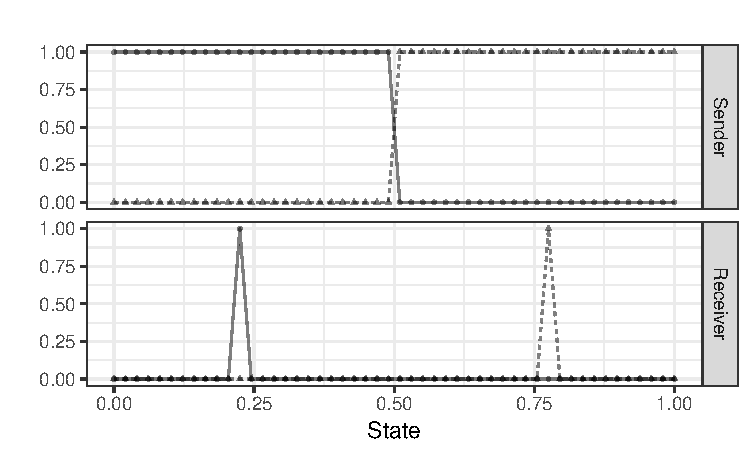
\includegraphics[width=\textwidth]{Rplot-example-strict.pdf}
    \caption{Crisp}
    \label{fig:example_stratsA}
  \end{subfigure}
  \hfill
  \begin{subfigure}[]{0.45\textwidth}
    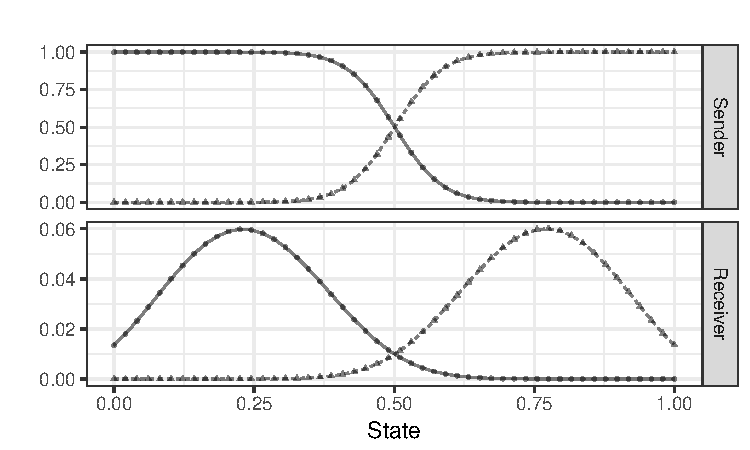
\includegraphics[width=\textwidth]{Rplot-example-vague.pdf}
    \caption{Vague}
    \label{fig:example_stratsB}
  \end{subfigure}

  \caption{Example strategies for a state space with 50 states. Each line corresponds to a message. For the sender, it plots for each state the probability that the message is used. For the receiver, it plots for each state the probability that the response is that state, given the message.}
  \label{fig:example_strats}
\end{figure}

In an abstract setup, using 50 states uniformly distributed over the unit interval and two possible messages, such an optimal language looks like what we see in Figure~\ref{fig:example_stratsA}.
The sender/receiver strategy pairs that we are looking for look more like Figure~\ref{fig:example_stratsB}.
While in the former the probability that the sender uses one message decays sharply from 1 to 0, and increases sharply from 0 to 1 for the other message, at a given point, in the latter these transitions are smooth.
This means that, for some states in the middle of the state space, there is uncertainty as to which message will be used, whereas for states in the extremes this is almost certain.
Similarly for the receiver strategy, in the first example for each message there is an almost certain response, whereas in the second example this is a degree of uncertainty.

The interpretation of this uncertainty will be different depending on the interpretation of the model.
If we see it as an explanatory model of how two agents play the game, we can see it as randomization.
If we interpret the model as descriptive, it simply represents expected behavior in a manner agnostic to the underlying mechanisms.
A third option is to see probabilities as capturing relative numbers in a population of agents.
For example, if the sender strategy assigns a probability of $0.4$ of message $m$ being sent for state $t$, this would mean that $40\%$ of the population uses that message for that state, while $60\%$ uses the other.
This latter option leaves open the possible interpretation that each agent commands a crisp language and vagueness is only a population-level effect.
However, given the level of abstraction of the description so far, none of this is necessarily implied by the model.

Our question is thus what additional modifications to sim-max games are sufficient for the optimal languages to be more like Figure~\ref{fig:example_stratsB}, rather than like Figure~\ref{fig:example_stratsA}.
Let's look at some proposals in the literature.

\subsection{Bounded rationality}
\textcite{franke_vagueness_2011} make two suggestions of how vagueness in a signaling game can arise as a consequence of limitations in the cognitive capacities of rational agents.
The first proposal is called limited memory fictitious play (LMF) and models agents playing a sim-max game where their ability to recall past interactions with others is limited to a certain number.
For a given interaction, each agent uses his limited memory of the other agent's past behavior to estimate the other's strategy.
Agents are assumed to be rational, thus each plays a best response (given the utility function) to their estimate of the other's strategy.
In order to observe the evolution of strategies in repeated interaction, this approach involves modeling several individual agents in actual play.
What the authors observe is the emergence of vague signaling at the level of the population, \emph{i.e.}~population averages of individual strategies exhibit the characteristics of a vague language as characterized before.
However, each agent still commands a crisp language, which is inadequate if the intention is to capture how vagueness presents itself in human languages.

In order to overcome this limitation, they make another proposal using the notion of a quantal response equilibrium (QRE).
The idea, inspired by experimental psychology, is to model the choice of best response as stochastic rather than deterministic, deviating from the optimal according to an exponentially decaying distribution (where small deviations are very likely, and large ones very rare).
The approach is not explanatory but descriptive: it is assumed that agents are not always able to make the absolute best choice, but the mechanism behind this limitation is left open to interpretation.
The degree to which agents deviate from the optimal behavior can be characterized by a parameter.
The authors find that for low values of this parameter, only babbling equilibria (where sender and receiver simply randomize, respectively, message and response uniformly) where no communication actually occurs.
Above a certain value of the parameter, other equilibria of the kind described in the beginning of this section arise, where agents communicate successfully, though not perfectly, using fuzzy strategies similar to the ones depicted in Figure~\ref{fig:example_stratsB}.


\subsection{Generalized reinforcement learning}
Cailin O'Connor~\parencite*{oconnor_evolution_2014} proposes a way in which vagueness could be expected to evolve as a side-effect of a particular type of learning process.
She studies sim-max games driven not by rational choice dynamics, but by generalized reinforcement learning (GRL), a variant of Herrnstein reinforcement learning (HRL)~\parencite{roth_learning_1995}.
In HRL, agents learn to play a signaling game by strengthening particular choices (of messages for the sender, of responses for the receiver) proportionally to how successful that choice proves to be in an interaction.
O'Connor's proposal is to model generalization as the propagation of reinforcement to nearby states, where ``nearby'' is defined in terms of distance in state space.
For example, if a sender was successful in using message $m$ for state $t$, he will not only positively reinforce that choice of message for $t$, but also for states similar to $t$.
This is done in a degree that is proportional to the degree of similarity between $t$ and other states.
The dynamics also gives rise to vague signaling of the kind we are looking for.

But why should agents evolve to generalize?
%First, it is not argued that vagueness in itself is beneficial, but that it is a by-product of a learning mechanism.
O'Connor suggests that, despite a vague language having lower expected utility than a precise one, the learning mechanism that induces vagueness does have evolutionary advantages, though not obvious ones (see \textcite{oconnor_evolving_2015} for the detailed argument).
Considerations of optimality of strategies are typically made in terms of hypothetical atemporal comparisons of expected utility.
However, generalized reinforcement learning has an interesting property in comparison with more strict learning mechanisms: it achieves higher payoffs in a smaller period of time.
In a naturalized evolutionary setting this temporary advantage should also be taken into account.
Imagine an initial population of agents with random strategies, some using GRL and others using classical Herrnstein reinforcement learning to adapt to each other.
Although the latter type of agent can hypothetically develop a precise and more efficient signaling system, agents using GRL would coordinate on vague signaling strategies with high (though not optimal) expected utility sooner than agents using HRL.
In such a scenario, they could drive the other agents to extinction before the latter had time to achieve coordination and reap the benefits of a more precise signaling system.

But would such a language be stable?
In terms of evolutionary game theory, one could argue that a small enough group of mutants playing a precise signaling system could later invade a population of vague signalers.
There is, an additional advantage to the generalized learning that is relevant here, namely the ability to adapt to a changing environment.
Analysis of a game in terms of evolutionary stable states works well if we assume that the environment where the agents interact remains static.
However, in a more realistic setting this is not the case.
In a dynamic game with a variable environment, an ability to converge faster could give an evolutionary advantage over strict learning rules: as soon as the state space or the utiliry function change, GRL would quickly adapt and again potentially drive more strict learning mechanisms to extinction because of their short-term gains.


\subsection{Noisy perception}
\parencite{correia_bivalent_2013,franke_vagueness_2017}

\subsection{Preference misalignment}
\todo[inline]{Test CS~\parencite{crawford_strategic_1982} results in our model by using bias in utility function. READ Förster, M., and Riedel, F. (2011). Distorted Voronoi languages (working Paper). -> distorted Voronoi languages, i.e. shifted according to bias, but still crisp}

\subsection{Noisy communication}
\todo[inline]{Test if noise in communication channel as modeled by Blume~\parencite{blume_intentional_2014} induces vague strategies as well}


\printbibliography

\end{document}
